% Created 2020-10-26 lun 16:00
% Intended LaTeX compiler: pdflatex
\documentclass[presentation,aspectratio=1610]{beamer}
\usepackage[utf8]{inputenc}
\usepackage[T1]{fontenc}
\usepackage{graphicx}
\usepackage{grffile}
\usepackage{longtable}
\usepackage{wrapfig}
\usepackage{rotating}
\usepackage[normalem]{ulem}
\usepackage{amsmath}
\usepackage{textcomp}
\usepackage{amssymb}
\usepackage{capt-of}
\usepackage{hyperref}
\usepackage{khpreamble}
\usepackage{pgfplots}
\usepackage{pdfpages}
\usepackage{circuitikz}
\usepgfplotslibrary{groupplots}
\usetikzlibrary{positioning,circuits.plc.ladder}
\renewcommand*{\not}[1]{\ensuremath{\bar{#1}}}
\renewcommand*{\not}[1]{\ensuremath{\overline{#1}}}
\newcommand*{\coil}[1]{to[short] ++(0.5, 0) node[coordinate] (orig) {} arc [start angle=180, end angle=150,radius=8mm] (orig) arc [start angle=180, end angle=210,radius=8mm] (orig) ++(1cm, 0) node[coordinate] (coilend) {} arc [start angle=0, end angle=30,radius=8mm] (coilend) arc [start angle=0, end angle=-30,radius=8mm] (coilend) to[short] ++(0.5cm, 0) (orig) ++(0.5, 0.8) node {#1}}
\newcommand*{\etimer}[2]{to[short] node[coordinate, pos=1.0] (orig) {} ++(0.5, 0) ++(0, -5mm) rectangle ++(5mm ,10mm)   (orig)  ++(0, -10mm) node[coordinate] (corner1) {} rectangle ++(5mm,5mm) node[coordinate] (corner2) {} (corner1) to (corner2) (orig) ++(0mm,-5mm) to ++(5mm,-5mm) (orig) ++(5mm, 0) to[short] ++(5mm, 0) (orig) ++(2.5mm, 8mm) node {#1} (orig) ++(2.5mm, 0) node{#2}}
\makeatletter
%% Push Button
\pgfcircdeclarebipole{}{\ctikzvalof{bipoles/pushbutton/height 2}}{pushedbutton}{\ctikzvalof{bipoles/pushbutton/height}}{\ctikzvalof{bipoles/pushbutton/width}}{
\pgfsetlinewidth{\pgfkeysvalueof{/tikz/circuitikz/bipoles/thickness}\pgfstartlinewidth}
\pgf@circ@res@temp=-\pgfkeysvalueof{/tikz/circuitikz/nodes width}\pgf@circ@Rlen
\advance\pgf@circ@res@temp by -2\pgfstartlinewidth
\pgfpathmoveto{\pgfpoint{\pgf@circ@res@left}{\pgf@circ@res@temp}}
\pgfpathlineto{\pgfpoint{\pgf@circ@res@right}{\pgf@circ@res@temp}}
\pgfpathmoveto{\pgfpoint{0}{\pgf@circ@res@temp}}
\pgfpathlineto{\pgfpoint{0}{\pgf@circ@res@up}}
\pgfusepath{draw}
\pgftransformshift{\pgfpoint{\pgf@circ@res@left}{0pt}}
\pgfnode{ocirc}{center}{}{}{\pgfusepath{draw}}
\pgftransformshift{\pgfpoint{2\pgf@circ@res@right}{0pt}}
\pgfnode{ocirc}{center}{}{}{\pgfusepath{draw}}
}
\def\pgf@circ@pushedbutton@path#1{\pgf@circ@bipole@path{pushedbutton}{#1}}
\compattikzset{pushed button/.style = {\circuitikzbasekey, /tikz/to path=\pgf@circ@pushedbutton@path, l=#1}}
\makeatother
\usetheme{default}
\author{Kjartan Halvorsen}
\date{\today}
\title{Logic control of electro-pneumatic systems}
\hypersetup{
 pdfauthor={Kjartan Halvorsen},
 pdftitle={Logic control of electro-pneumatic systems},
 pdfkeywords={},
 pdfsubject={},
 pdfcreator={Emacs 26.3 (Org mode 9.3.6)}, 
 pdflang={English}}
\begin{document}

\maketitle

\section{Intro}
\label{sec:orgcdcd0d1}


\section{Logic control and boolean algebra - simple intro example}
\label{sec:orgfcfb1f8}
\begin{frame}[label={sec:orgff18f6d}]{Cheese pressing example, sequence A+A-}
\begin{center}
\includegraphics[width=0.5\linewidth]{../../figures/cheese-stamping.png}
\end{center}
{\tiny From FESTO Didactic}
\end{frame}

\begin{frame}[label={sec:orgea6201f}]{They Relay}
\begin{center}
\begin{tabular}{cc}
\includegraphics[width=0.4\linewidth]{../../figures/howrelayswork.jpg} &
\includegraphics[width=0.3\linewidth]{../../figures/festo-relay-principle.png}\\
{\tiny From pcbheaven.com} & {\tiny From FESTO didactic}\\
\includegraphics[width=0.35\linewidth]{../../figures/festo-relay-switches.png} &
\includegraphics[width=0.25\linewidth]{../../figures/festo-relay-box.jpg}\\
{\tiny From FESTO didactic} & {\tiny From FESTO didactic}\\
\end{tabular}
\end{center}
\end{frame}

\begin{frame}[label={sec:orga6ef96f}]{Other key components}
{\tiny Sources: FESTO didactic, electroschematics.com, automation-insights.blog}
\begin{columns}
\begin{column}{0.33\columnwidth}
\begin{block}{Limit switch}
\begin{center}
\includegraphics[width=0.4\linewidth]{../../figures/festo-mech-valve-symbol.png}\\
\includegraphics[width=0.3\linewidth]{../../figures/festo-limit-switch.jpg}\\
\includegraphics[width=0.5\linewidth]{../../figures/festo-mech-valve-section.png}\\
\end{center}
\end{block}
\end{column}


\begin{column}{0.33\columnwidth}
\begin{block}{Solenoid valve}
\begin{center}
\includegraphics[width=0.7\linewidth]{../../figures/festo-solenoid-52-symbol.png}\\
\includegraphics[width=0.45\linewidth]{../../figures/festo-solenoid-52.jpg}\\
\includegraphics[width=1.1\linewidth]{../../figures/festo-solenoid-schematic.png}\\
\end{center}
\end{block}
\end{column}
\begin{column}{0.33\columnwidth}
\begin{block}{Proximity sensor}
\includegraphics[width=0.4\linewidth]{../../figures/festo-inductive-sensor.png}\\
\includegraphics[width=0.6\linewidth]{../../figures/festo-proximity-sensor.jpg}\\
\includegraphics[width=0.99\linewidth]{../../figures/electroschematics-inductive-proximity-sensor.png}\\
\includegraphics[width=0.99\linewidth]{../../figures/automation-insight-operation_capacitive.jpg}
\end{block}
\end{column}
\end{columns}
\end{frame}


\begin{frame}[label={sec:orga327086}]{A logic control loop}
\begin{center}
\includegraphics[width=\linewidth]{../../figures/logic-control-loop}
\end{center}
\end{frame}

\begin{frame}[label={sec:org51f1787}]{Cheese pressing example - Variables}
\begin{columns}
\begin{column}{0.5\columnwidth}
\begin{block}{State variables}
\(x = \begin{bmatrix} x_R & x_R \end{bmatrix}^T\) with
\begin{align*}
x_R &= \begin{cases} 1 & \text{Cylinder retracted}\\0 & \text{not retracted}\end{cases}\\
x_E &= \begin{cases} 1 & \text{Cylinder extended}\\0 & \text{not extended}\end{cases}
\end{align*}
\end{block}
\begin{block}{Control signal}
\(u = \begin{bmatrix} u_1 & u_2 \end{bmatrix}^T,\) with
\begin{align*}
u_1 &= \begin{cases} 1 & \text{Activate UA+}\\0 & \text{Don't activate UA+ }\end{cases}\\
u_2 &= \begin{cases} 1 & \text{Activate UA-}\\0 & \text{Don't activate UA-}\end{cases}
\end{align*}
\end{block}
\end{column}

\begin{column}{0.5\columnwidth}
    \includegraphics[width=0.6\linewidth]{../../figures/AplAmin-solenoids.png}
Activating solenoid UA+ extends the cylinder, activating  UA- retracts the cylinder.
\begin{block}{Command signal}
\[ u_{c} = \begin{cases} 0 & \text{Button unpushed}\\1 & \text{Button pushed}\end{cases}. \]
\end{block}
\end{column}
\end{columns}
\end{frame}
\begin{frame}[label={sec:orgbf3e172}]{Cheese pressing example - Plant dynamics}
\begin{block}{Plant dynamics \(x_{k+1} = g(x_k, u_k)\)}
\begin{center}
\begin{tabular}{|cc|cc|cc|}
\hline
Input &  & Current state &  & Next state & \\
\(u_{1,k}\) & \(u_{2,k}\) & \(x_{R,k}\) & \(x_{E, k}\) & \(x_{R,k+1}\) & \(x_{E,k+1}\)\\
 &  &  &  &  & \\
\hline
0 & 0 & 0 & 1 & 0 & 1\\
0 & 1 & 0 & 1 & 1 & 0\\
1 & 0 & 0 & 1 & 0 & 1\\
(1) & (1) & (0) & (1) & (0) & (1)\\
0 & 0 & 1 & 0 & 1 & 0\\
0 & 1 & 1 & 0 & 1 & 0\\
1 & 0 & 1 & 0 & 0 & 1\\
(1) & (1) & (1) & (0) & (1) & (0)\\
\hline
\end{tabular}
\end{center}
\end{block}
\end{frame}
\begin{frame}[label={sec:org85c4b53}]{Intermezzo - Maxterms and minterms}
\end{frame}
\begin{frame}[label={sec:org2613159}]{Minterms}
\alert{A minterm is a boolean expression that is TRUE (=1) for one and only one row in the truth table.} For instance \(Y=X_1X_2X_3\) will only be true when \(X_1=X_2=X_3=1\), and \(Y=\not{X_1}X_2\not{X_3}\) will only be true if \(X_1=X_3=0\) and \(X_2=1\). The combination \(Y=X_1X_2X_3 + \not{X_1}X_2\not{X_3}\) will have \alert{only two rows} equal to 1 in the truth table.   

Example:
\begin{center}
\begin{tabular}{|ccc|cc|}
\hline
Inputs &  &  & Outputs & \\
\(X_1\) & \(X_2\) & \(X_3\) & \(Y_1\) & \(Y_2\)\\
\hline
0 & 0 & 0 & 0 & 1\\
0 & 0 & 1 & 0 & 0\\
0 & 1 & 0 & 1 & 0\\
0 & 1 & 1 & 1 & 0\\
1 & 0 & 0 & 0 & 0\\
1 & 0 & 1 & 0 & 0\\
1 & 1 & 0 & 0 & 0\\
1 & 1 & 1 & 0 & 1\\
\hline
\end{tabular}
\end{center}

\(Y_1 = m_2 + m_3 = \not{X_1}X_2\not{X_3} + \not{X_1}X_2X_3, \qquad   Y_2 =\) 
\end{frame}


\begin{frame}[label={sec:orge3a3622}]{Maxterms}
\alert{A maxterm is a boolean expression that is FALSE (=0) for one and only one row in the truth table.} For instance \(Y=X_1+X_2+X_3\) will only be false when \(X_1=X_2=X_3=0\), and \(Y=\not{X_1}+X_2+\not{X_3}\) will only be false if \(X_1=X_3=1\) and \(X_2=0\). The combination \(Y=(X_1+X_2+X_3)(\not{X_1}+X_2+\not{X_3})\) will have \alert{only two rows} equal to 0 in the truth table.   

Example:
\begin{center}
\begin{tabular}{|ccc|cc|}
\hline
Inputs &  &  & Outputs & \\
\(X_1\) & \(X_2\) & \(X_3\) & \(Y_1\) & \(Y_2\)\\
\hline
0 & 0 & 0 & 0 & 1\\
0 & 0 & 1 & 0 & 1\\
0 & 1 & 0 & 1 & 1\\
0 & 1 & 1 & 1 & 1\\
1 & 0 & 0 & 1 & 1\\
1 & 0 & 1 & 1 & 1\\
1 & 1 & 0 & 1 & 0\\
1 & 1 & 1 & 1 & 0\\
\hline
\end{tabular}
\end{center}


\(Y_1 = M_0M_1 = (X_1+X_2+X_3)(X_1+X_2+\not{X_3}), \qquad   Y_2 =\) 
\end{frame}



\begin{frame}[label={sec:org75c3d14}]{Cheese pressing example - Control law}
The system is operating as long as the start button is pressed (\(u_c=1\)). When the button is released, the cylinder should go to the retracted position.
\begin{block}{Control law \(u_k = f(x, u_c)\)}
\begin{center}
\begin{tabular}{|ccc|cc|}
\hline
\(x_R\) & x\textsubscript{E} & \(u_{c}\) & \(u_1\) & \(u_2\)\\
\hline
0 & 1 & 0 & 0 & 1\\
1 & 0 & 0 & 0 & 0\\
0 & 1 & 1 & 0 & 1\\
1 & 0 & 1 & 1 & 0\\
0 & 0 & 0 & 0 & 1\\
0 & 0 & 1 & 0 & 0\\
\hline
\end{tabular}
\end{center}

\alert{Activity:} Write as boolen functions
\begin{align*}
  u_1 &= f_1(x_R, x_E, u_c) = \qquad\qquad\quad\\
  u_2 &= f_2(x_R, x_E, u_c) =
\end{align*}
\end{block}
\end{frame}
\begin{frame}[label={sec:org7e607ee}]{Cheese pressing example - implementing the control  law}
\begin{center}
	 \begin{tikzpicture}
	   \node at (-2,0.5) {+24V};
	   \node at (8,0.5) {0V};
	   \draw (-2,0) to[short, o-]  (-2,-3);
	   \draw (8,0) to[short, o-](8,-3);
	   \draw (6, -0.5) \coil{$u_1$};
	   \draw (6,-2.5) \coil{$u_2$};
      \end{tikzpicture}
\end{center}
\begin{center}
  \begin{tikzpicture}
    \draw(0,0) to [push button, label={normally open}] ++(2,0);
    \draw(5,0) to [pushed button, label={normally closed}] ++(2,0);
  \end{tikzpicture}
\end{center}
\begin{center}
  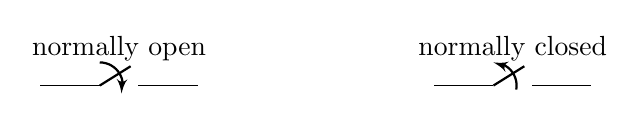
\begin{tikzpicture}
    \draw(0,0) to [switch, label={normally open}] ++(2,0);
    \draw(5,0) to [opening switch, label={normally closed}] ++(2,0);
  \end{tikzpicture}
\end{center}
\begin{center}
  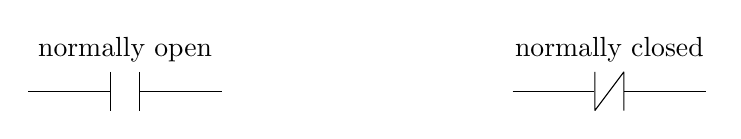
\begin{tikzpicture}[circuit plc ladder,]
    \draw(0,0) to [contact NO={info={normally open}}] ++(2,0);
    \draw(5,0) to [contact NC={info={normally closed}}] ++(2,0);
  \end{tikzpicture}
\end{center}
\end{frame}

\section{Latching circuit}
\label{sec:orgf584dcf}
\begin{frame}[label={sec:org459c718}]{Intermezzo - An electrical circuit with memory}
\begin{center}
\begin{tabular}{cc}
\includegraphics[width=0.4\linewidth]{../../figures/howrelayswork.jpg} &
\includegraphics[width=0.3\linewidth]{../../figures/festo-relay-principle.png}\\
{\tiny From pcbheaven.com} & {\tiny From FESTO didactic}\\
\includegraphics[width=0.35\linewidth]{../../figures/festo-relay-switches.png} &
\includegraphics[width=0.25\linewidth]{../../figures/festo-relay-box.jpg}\\
{\tiny From FESTO didactic} & {\tiny From FESTO didactic}\\
\end{tabular}
\end{center}
\end{frame}

\begin{frame}[label={sec:org701a217}]{Intermezzo - An electrical circuit with memory}
\begin{columns}
\begin{column}{0.6\columnwidth}
\begin{block}{Latching circuit}
\begin{center}
         \begin{tikzpicture}
           \node at (0,0.5) {+24V};
           \node at (6,0.5) {0V};
           \draw (0,0) to[short, o-]  (0,-2.5);
           \draw (6,0) to[short, o-](6,-2.5);
           \draw (0,-0.3) to[push button, label={$X$}] (2,-0.3) to[pushed button, label=$Y$, ] (4,-0.3) to[short] (4,-0.3) to[twoport, label={$R$}] (6,-0.3); %\coil{$R$};
           \draw (0,-2) to[switch,label={$R$}] (2,-2)  to[short] (2,-0.3);
         \end{tikzpicture}
\end{center}
\begin{center}
         \begin{tikzpicture}[circuit plc ladder,]
           \node at (0,0.5) {+24V};
           \node at (6,0.5) {0V};
           \draw (0,0) to[short, o-]  (0,-2.5);
           \draw (6,0) to[short, o-](6,-2.5);
           \draw (0,-0.3) to[contact NO={info={$X$}},] (2,-0.3) to[ contact NC={info={$Y$}}, ] (4,-0.3) to[short] (4,-0.3) \coil{$R$};
           \draw (0,-2) to[contact NO={info={$R$}},] (2,-2)  to[short,] (2,-0.3);
         \end{tikzpicture}
\end{center}
\end{block}
\end{column}


\begin{column}{0.4\columnwidth}
\begin{block}{Truth table}
\begin{center}
\begin{tabular}{|ccc|c|}
\(X\) & \(Y\) & \(R_k\) & \(R_{k+1}\)\\
\hline
0 & 0 & 0 & \\
0 & 0 & 1 & \\
0 & 1 & 0 & \\
0 & 1 & 1 & \\
1 & 0 & 0 & \\
1 & 0 & 1 & \\
1 & 1 & 0 & \\
1 & 1 & 1 & \\
\hline
\end{tabular}
\end{center}

\alert{Group activity:} Implement the circuit in FluidSim and verify the truth table.
\end{block}
\end{column}
\end{columns}
\end{frame}

\begin{frame}[label={sec:orga7fd13e}]{Electrical circuits in FluidSim}
\begin{center}
\includegraphics[width=0.9\linewidth]{../../figures/fluidsim-ladder.png}
\end{center}
\end{frame}

\section{The lab assignment}
\label{sec:orgc58c296}


\begin{frame}[label={sec:orgb52ad6b}]{The lab assignment}
\begin{center}
\includegraphics[width=0.4\linewidth]{../../figures/cheese-pressing-two-cylinders}
 \includegraphics[width=0.58\linewidth]{../../figures/AplusBplusBminAmin}
\end{center}

\begin{center}
\includegraphics[width=0.8\linewidth]{../../figures/logic-control-loop}
\end{center}
\end{frame}

\begin{frame}[label={sec:orgc4fa9cd}]{Implementing the sequence A+B+B-A-}
\begin{center}
\includegraphics[width=0.8\linewidth]{../../figures/AplusBplusBminAmin}
\end{center}
\end{frame}

\begin{frame}[label={sec:orgf95b987}]{Implementing the sequence A+B+B-A-, control signal}
\begin{center}
\includegraphics[width=0.42\linewidth]{../../figures/AplBplBminAmin-pneum.png}
\includegraphics[width=0.58\linewidth]{../../figures/logic-control-loop}
\end{center}

\begin{block}{Control signal}
\[ u = \begin{bmatrix} u_A+ & u_A- & u_B+ & u_B- \end{bmatrix}^T, \]
with
\[ u_A+ = \begin{cases} 0 & \text{Solenoid extending A is not activated}\\
                               1&\text{Solenoid extending A is activated}\\
              \end{cases}, \qquad \text{and similar for B}
   \]
\end{block}
\end{frame}

\begin{frame}[label={sec:org65632f8}]{Implementing the sequence A+B+B-A-, the problem}
\alert{The correct control signal (action) is not uniquely defined by the position of the cylinders}
\begin{center}
\includegraphics[width=0.5\linewidth]{../../figures/AplusBplusBminAmin}\\
\includegraphics[width=0.8\linewidth]{../../figures/logic-control-loop}
\end{center}
\end{frame}

\begin{frame}[label={sec:org5280cce}]{Implementing the sequence A+B+|B-A-}
\alert{Dividing the sequence into groups (a.k.a. cascade method)} Each group contains as many steps as possible without repeating a letter.
\[ \underbrace{\text{A+B+}}_{\text{Group 1}}| \underbrace{\text{B-A-}}_{\text{Group 2}} \]
 \begin{center}
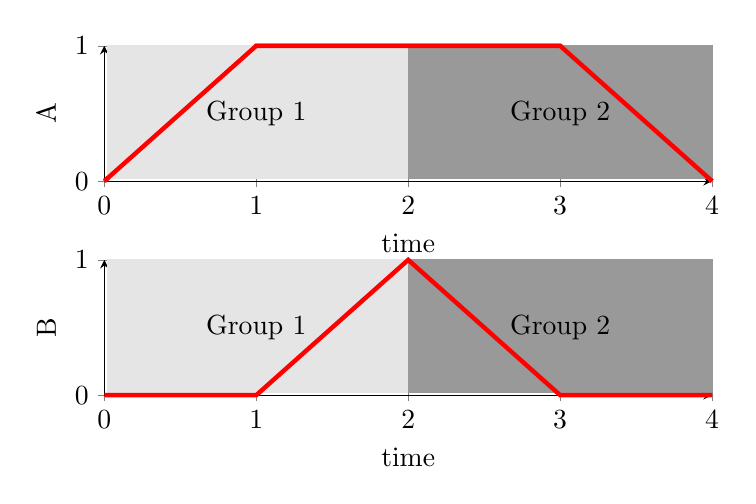
\begin{tikzpicture}
%\pgfplotsset{set layers=default}
  \begin{groupplot} [
    group style={
      group name=timeplot,
      group size=1 by 2,
      xlabels at=all,
      horizontal sep=1cm,
      vertical sep=1cm,
    }, 
    clip=false,
    height=3.3cm, width=9.3cm,
    axis line style={->},
    axis lines=left,
    xlabel={time },
    ylabel={},
    ytick={0,1},
    xtick={0,1,2,3,4},
    % grid=both,
    % xtick=\empty,
    % ytick=\XNOLL,
    % yticklabel=$x_0$,
    ]
    \nextgroupplot [ylabel={A},]
    \addplot[red, no marks,ultra thick,] coordinates {(0,0) (1,1) (2, 1) (3,1) (4, 0)};
    \draw[color=black!10, fill=black!10] (axis cs: 0.02,0.02) rectangle (axis cs: 2,1);
    \node at (axis cs: 1, 0.5) {Group 1};
    \draw[color=black!40, fill=black!40] (axis cs: 2,0.02) rectangle (axis cs: 4,1);
    \node at (axis cs: 3, 0.5) {Group 2};
    \addplot[red, no marks,ultra thick,] coordinates {(0,0) (1,1) (2, 1) (3,1) (4, 0)};

    \nextgroupplot [ylabel={B},]
    \draw[color=black!10, fill=black!10] (axis cs: 0.02,0.02) rectangle (axis cs: 2,1);
    \node at (axis cs: 1, 0.5) {Group 1};
    \draw[color=black!40, fill=black!40] (axis cs: 2,0.02) rectangle (axis cs: 4,1);
    \node at (axis cs: 3, 0.5) {Group 2};
    \addplot[red, no marks,ultra thick,] coordinates {(0,0) (1,0) (2, 1) (3,0) (4, 0)};
  \end{groupplot}
\end{tikzpicture}
  \end{center}
\end{frame}

\section{Cascade method for A+A-}
\label{sec:org9bb80ed}
\begin{frame}[label={sec:org07b67f6}]{The cascade method applied to A+A-}
\end{frame}

\begin{frame}[label={sec:orgb6e5c7b}]{The cascade method applied to A+A-}
Divide the sequence is to groups, where each group is as long as possible without repeating the same letter.
\[ \underbrace{\text{A+}}_{\text{Group 1}}| \underbrace{\text{A-}}_{\text{Group 2}} \]
 \begin{center}
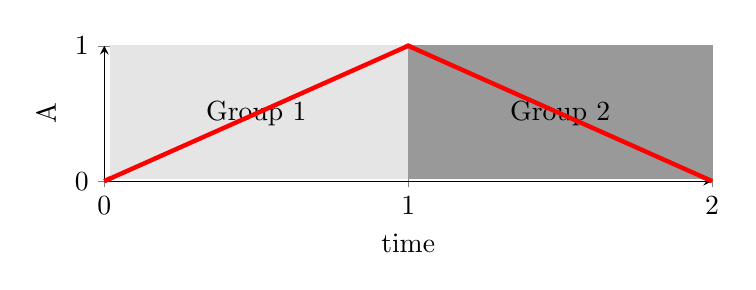
\begin{tikzpicture}
%\pgfplotsset{set layers=default}
  \begin{groupplot} [
    group style={
      group name=timeplot,
      group size=1 by 1,
      xlabels at=all,
      horizontal sep=1cm,
      vertical sep=1cm,
    }, 
    clip=false,
    height=3.3cm, width=9.3cm,
    axis line style={->},
    axis lines=left,
    xlabel={time },
    ylabel={},
    ytick={0,1},
    xtick={0,1,2},
    % grid=both,
    % xtick=\empty,
    % ytick=\XNOLL,
    % yticklabel=$x_0$,
    ]
    \nextgroupplot [ylabel={A},]
    \addplot[red, no marks,ultra thick,] coordinates {(0,0) (1,1) (2, 0)};
    \draw[color=black!10, fill=black!10] (axis cs: 0.02,0.02) rectangle (axis cs: 1,1);
    \node at (axis cs: 0.5, 0.5) {Group 1};
    \draw[color=black!40, fill=black!40] (axis cs: 1,0.02) rectangle (axis cs: 2,1);
    \node at (axis cs: 1.5, 0.5) {Group 2};
    \addplot[red, no marks,ultra thick,] coordinates {(0,0) (1,1) (2, 0)};

  \end{groupplot}
\end{tikzpicture}
  \end{center}
\end{frame}

\begin{frame}[label={sec:org1f4ec65}]{The cascade method applied to A+A- with delays}
Let's add some delays. The process is cyclic and automatic. It takes 4 seconds to replace the mold under the press. The cheese needs to be pressed during 2 seconds before the cylinder retracts. 
\[ \underbrace{T_{4s} \, \text{A+}}_{\text{Group 1}}| \underbrace{T_{2s}\, \text{A-} }_{\text{Group 2}} \]
 \begin{center}
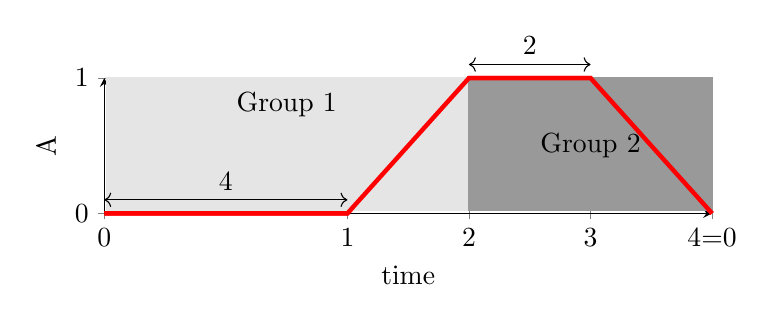
\begin{tikzpicture}
%\pgfplotsset{set layers=default}
  \begin{groupplot} [
    group style={
      group name=timeplot,
      group size=1 by 1,
      xlabels at=all,
      horizontal sep=1cm,
      vertical sep=1cm,
    }, 
    clip=false,
    height=3.3cm, width=9.3cm,
    axis line style={->},
    axis lines=left,
    xlabel={time },
    ylabel={},
    ytick={0,1},
    xtick={0,2,3,4,5},
    xticklabels={0,1,2,3,4=0},
    % grid=both,
    % xtick=\empty,
    % ytick=\XNOLL,
    % yticklabel=$x_0$,
    ]
    \nextgroupplot [ylabel={A},]
    \addplot[red, no marks,ultra thick,] coordinates {(0,0) (2,0) (3,1) (4,1) (5, 0)};
    \draw[color=black!10, fill=black!10] (axis cs: 0.02,0.02) rectangle (axis cs: 3,1);
    \node at (axis cs: 1.5, 0.8) {Group 1};
    \draw[color=black!40, fill=black!40] (axis cs: 3,0.02) rectangle (axis cs: 5,1);
    \node at (axis cs: 4, 0.5) {Group 2};
    \addplot[red, no marks,ultra thick,] coordinates {(0,0) (2,0) (3,1) (4,1) (5, 0)};
    \draw[<->] (axis cs: 0, 0.1) -- node[above] {\unit{4}{\second}} (axis cs: 2, 0.1);
    \draw[<->] (axis cs: 3, 1.1) -- node[above] {\unit{2}{\second}} (axis cs: 4, 1.1);


  \end{groupplot}
\end{tikzpicture}
  \end{center}
\end{frame}


\begin{frame}[label={sec:orge245dca}]{State variables}
\begin{columns}
\begin{column}{0.45\columnwidth}
\begin{block}{State variables}
\[ x = \begin{bmatrix} x_R & x_E & x_{G1} & x_{G2} & x_{T4} & x_{T2}\end{bmatrix}^T, \]
where
 \begin{align*}
  x_{R} &= \begin{cases} 1 & \text{Cylinder A retracted}\\
                            0& \text{not retracted}
              \end{cases}\\
  x_{E} &= \begin{cases} 1 & \text{Cylinder A extended}\\
                            0& \text{not extended}
              \end{cases}\\
 x_{Gi} &= \begin{cases} 1 & \text{Group \(i\) active}\\
                            0& \text{Group \(i\) not active}
              \end{cases}\\
 x_{Ti} &= \begin{cases} 1 & \text{Timer of \(i\) s  completed}\\
                            1& \text{Timer of \(i\)s not completed}
              \end{cases}
\end{align*}
\end{block}
\end{column}

\begin{column}{0.55\columnwidth}
\begin{block}{State transitions}
 \begin{center}
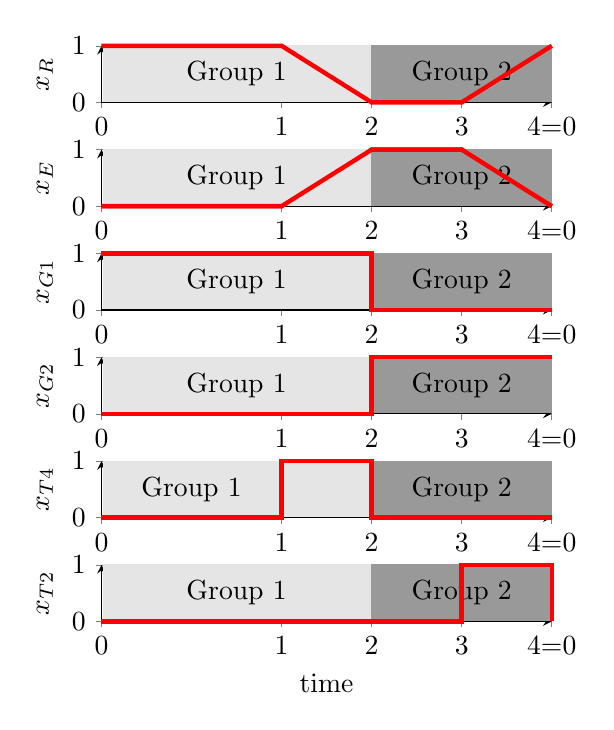
\begin{tikzpicture}
%\pgfplotsset{set layers=default}
  \begin{groupplot} [
    group style={
      group name=timeplot,
      group size=1 by 6,
      xlabels at=edge bottom,
      horizontal sep=1cm,
      vertical sep=6mm,
    }, 
    clip=false,
    height=2.3cm, width=7.3cm,
    axis line style={->},
    axis lines=left,
    xlabel={time },
    ylabel={},
    ytick={0,1},
    xtick={0,2,3,4,5},
    xticklabels={0,1,2,3,4=0},
    % grid=both,
    % xtick=\empty,
    % ytick=\XNOLL,
    % yticklabel=$x_0$,
    ]
    \nextgroupplot [ylabel={$x_R$},]
    \draw[color=black!10, fill=black!10] (axis cs: 0.02,0.02) rectangle (axis cs: 3,1);
    \node at (axis cs: 1.5, 0.5) {Group 1};
    \draw[color=black!40, fill=black!40] (axis cs: 3,0.02) rectangle (axis cs: 5,1);
    \node at (axis cs: 4, 0.5) {Group 2};
    \addplot[red, no marks,ultra thick,] coordinates {(0,1) (2,1) (3,0) (4,0) (5, 1)};

    \nextgroupplot [ylabel={$x_E$},]
    \addplot[red, no marks,ultra thick,] coordinates {(0,0) (2,0) (3,1) (4,1) (5, 0)};
    \draw[color=black!10, fill=black!10] (axis cs: 0.02,0.02) rectangle (axis cs: 3,1);
    \node at (axis cs: 1.5, 0.5) {Group 1};
    \draw[color=black!40, fill=black!40] (axis cs: 3,0.02) rectangle (axis cs: 5,1);
    \node at (axis cs: 4, 0.5) {Group 2};
    \addplot[red, no marks,ultra thick,] coordinates {(0,0) (2,0) (3,1) (4,1) (5, 0)};

    \nextgroupplot [ylabel={$x_{G1}$},]
    \draw[color=black!10, fill=black!10] (axis cs: 0.02,0.02) rectangle (axis cs: 3,1);
    \node at (axis cs: 1.5, 0.5) {Group 1};
    \draw[color=black!40, fill=black!40] (axis cs: 3,0.02) rectangle (axis cs: 5,1);
    \node at (axis cs: 4, 0.5) {Group 2};
    \addplot[red, no marks,ultra thick,] coordinates {(0,1) (3, 1) (3,0) (4, 0) (5,0)} ;

    \nextgroupplot [ylabel={$x_{G2}$},]
    \draw[color=black!10, fill=black!10] (axis cs: 0.02,0.02) rectangle (axis cs: 3,1);
    \node at (axis cs: 1.5, 0.5) {Group 1};
    \draw[color=black!40, fill=black!40] (axis cs: 3,0.02) rectangle (axis cs: 5,1);
    \node at (axis cs: 4, 0.5) {Group 2};
    \addplot[red, no marks,ultra thick,] coordinates {(0,0) (3, 0) (3,1) (4, 1) (5,1)};

    \nextgroupplot [ylabel={$x_{T4}$},]
    \draw[color=black!10, fill=black!10] (axis cs: 0.02,0.02) rectangle (axis cs: 3,1);
    \node at (axis cs: 1, 0.5) {Group 1};
    \draw[color=black!40, fill=black!40] (axis cs: 3,0.02) rectangle (axis cs: 5,1);
    \node at (axis cs: 4, 0.5) {Group 2};
    \addplot[red, no marks,ultra thick,] coordinates {(0,0) (2,0) (2, 1) (3, 1) (3,0) (5,0)};

    \nextgroupplot [ylabel={$x_{T2}$},]
    \draw[color=black!10, fill=black!10] (axis cs: 0.02,0.02) rectangle (axis cs: 3,1);
    \node at (axis cs: 1.5, 0.5) {Group 1};
    \draw[color=black!40, fill=black!40] (axis cs: 3,0.02) rectangle (axis cs: 5,1);
    \node at (axis cs: 4, 0.5) {Group 2};
    \addplot[red, no marks,ultra thick,] coordinates {(0,0) (4,0) (4, 1) (5, 1) (5,0)};

  \end{groupplot}
\end{tikzpicture}
  \end{center}
\end{block}
\end{column}
\end{columns}
\end{frame}

\begin{frame}[label={sec:org5a10650}]{Group transitions}
            \begin{center}
                     \begin{tikzpicture}
		     \pgfmathsetmacro\zrail{10}
		     \pgfmathsetmacro\cstart{\zrail -2}
		     \pgfmathsetmacro\pend{4}
                       \node at (0,0.5) {+24V};
                       \node at (\zrail,0.5) {0V};
                       \draw (0,0) to[short, o-]  (0,-7);
                       \draw (\zrail,0) to[short, o-](\zrail,-7);

                       \draw (0,-0.3) to[short] (2, -0.3) to[switch, label=$x_R$] (\pend,-0.3) to[ opening switch, label=$x_E$, ] ++(2,0) to[short] (\cstart,-0.3) \coil{$G_1$};
                       \draw (0,-2) to[switch, label=$G_1$] (\pend,-2)  to[short,] (\pend,-0.3);

%                       \draw (0,-3.3) to[short] (2,-3.3) to[switch, label=$x_A$] (\pend,-3.3) to[ opening switch, label=$\overline{x_A}$, ] ++(2,0) to[short] (\cstart,-3.3);
\draw (\cstart, -3.3) \coil{$G_2$};
%                       \draw (0,-5) to[switch, label=$G_2$] (\pend,-5)  to[short] (\pend,-3.3);
                     \end{tikzpicture}
            \end{center}
\end{frame}


\begin{frame}[label={sec:org1daaecc}]{The timers}
\begin{center}
         \begin{tikzpicture}
	 \pgfmathsetmacro\zrail{10}
	 \pgfmathsetmacro\cstart{\zrail -1.5}
	 \pgfmathsetmacro\pend{4}
	 \pgfmathsetmacro\rone{-1.3}
	 \pgfmathsetmacro\rtwo{-4.3}
           \node at (0,0.5) {+24V};
           \node at (\zrail,0.5) {0V};
           \draw (0,0) to[short, o-]  (0,-5);
           \draw (\zrail,0) to[short, o-](\zrail,-5);

           \draw (0,\rone) to[switch, label=$x_R$] (\pend,\rone) to[short,] (\cstart,\rone) \etimer{$T_{4}$}{4};
           \draw (0,\rtwo) to[switch, label=$x_A$] (\pend,\rtwo) to[short,] (\cstart,\rtwo) \etimer{$T_{2}$}{2};
         \end{tikzpicture}
\end{center}
\end{frame}

\begin{frame}[label={sec:org9ddb98b}]{The control law}
\begin{center}
         \begin{tikzpicture}
	 \pgfmathsetmacro\zrail{10}
	 \pgfmathsetmacro\cstart{\zrail -2}
	 \pgfmathsetmacro\pend{4}
	 \pgfmathsetmacro\rone{-1.3}
	 \pgfmathsetmacro\rtwo{-4.3}
           \node at (0,0.5) {+24V};
           \node at (\zrail,0.5) {0V};
           \draw (0,0) to[short, o-]  (0,-5);
           \draw (\zrail,0) to[short, o-](\zrail,-5);

           \draw (0,\rone) to[switch, label=$x_{G1}$] ++(2cm, 0) to [switch, label=$x_{T4}$] ++(2cm, 0) to[short,] (\cstart,\rone) \coil{$u_{A+}$};
           \draw (0,\rtwo) to[switch, label=$x_{G2}$] ++(2cm, 0) to [switch, label=$x_{T2}$] ++(2cm, 0) to[short,] (\cstart,\rtwo) \coil{$u_{A-}$};
         \end{tikzpicture}
\end{center}
\end{frame}



\section{Continue with lab assignment}
\label{sec:orge19ad7e}
\begin{frame}[label={sec:org2e6efcb}]{The lab assignment}
\begin{center}
\includegraphics[width=0.4\linewidth]{../../figures/cheese-pressing-two-cylinders}
 \includegraphics[width=0.58\linewidth]{../../figures/AplusBplusBminAmin}
\end{center}

\begin{center}
\includegraphics[width=0.8\linewidth]{../../figures/logic-control-loop}
\end{center}
\end{frame}

\begin{frame}[label={sec:orgf164847}]{Implementing the sequence A+B+|B-A-, state variables}
\begin{columns}
\begin{column}{0.45\columnwidth}
\begin{block}{State variables}
\[ x = \begin{bmatrix} A_R & A_E & B_R & B_E & G_1 & G_2\end{bmatrix}^T, \]
with
 \begin{align*}
  {\{A_R,B_R\}} &= \begin{cases} 1 & \text{\{A,B\} retracted}\\
                            0& \text{\{A,B\} not retracted }
              \end{cases}\\
  {\{A_E,B_E\}} &= \begin{cases} 1 & \text{\{A,B\} extended}\\
                            0& \text{\{A,B\} not extended }
              \end{cases}\\
 G_i &= \begin{cases} 0 & \text{Group \(i\) not active}\\
                            1& \text{Group \(i\) active}
              \end{cases}
\end{align*}
\end{block}
\end{column}

\begin{column}{0.55\columnwidth}
\begin{block}{State transitions}
 \begin{center}
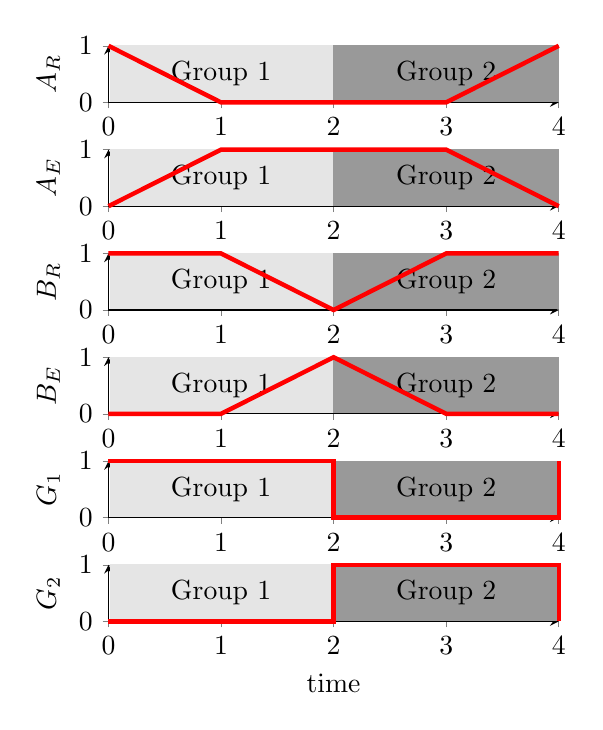
\begin{tikzpicture}
%\pgfplotsset{set layers=default}
  \begin{groupplot} [
    group style={
      group name=timeplot,
      group size=1 by 6,
      xlabels at=edge bottom,
      horizontal sep=1cm,
      vertical sep=6mm,
    }, 
    clip=false,
    height=2.3cm, width=7.3cm,
    axis line style={->},
    axis lines=left,
    xlabel={time },
    ylabel={},
    ytick={0,1},
    xtick={0,1,2,3,4},
    % grid=both,
    % xtick=\empty,
    % ytick=\XNOLL,
    % yticklabel=$x_0$,
    ]
    \nextgroupplot [ylabel={$A_R$},]
    \draw[color=black!10, fill=black!10] (axis cs: 0.02,0.02) rectangle (axis cs: 2,1);
    \node at (axis cs: 1, 0.5) {Group 1};
    \draw[color=black!40, fill=black!40] (axis cs: 2,0.02) rectangle (axis cs: 4,1);
    \node at (axis cs: 3, 0.5) {Group 2};
    \addplot[red, no marks,ultra thick,] coordinates {(0,1) (1,0) (2, 0) (3,0) (4, 1)};

    \nextgroupplot [ylabel={$A_E$},]
    \draw[color=black!10, fill=black!10] (axis cs: 0.02,0.02) rectangle (axis cs: 2,1);
    \node at (axis cs: 1, 0.5) {Group 1};
    \draw[color=black!40, fill=black!40] (axis cs: 2,0.02) rectangle (axis cs: 4,1);
    \node at (axis cs: 3, 0.5) {Group 2};
    \addplot[red, no marks,ultra thick,] coordinates {(0,0) (1,1) (2, 1) (3,1) (4, 0)};

    \nextgroupplot [ylabel={$B_R$},]
    \draw[color=black!10, fill=black!10] (axis cs: 0.02,0.02) rectangle (axis cs: 2,1);
    \node at (axis cs: 1, 0.5) {Group 1};
    \draw[color=black!40, fill=black!40] (axis cs: 2,0.02) rectangle (axis cs: 4,1);
    \node at (axis cs: 3, 0.5) {Group 2};
    \addplot[red, no marks,ultra thick,] coordinates {(0,1) (1,1) (2, 0) (3,1) (4, 1)};

    \nextgroupplot [ylabel={$B_E$},]
    \draw[color=black!10, fill=black!10] (axis cs: 0.02,0.02) rectangle (axis cs: 2,1);
    \node at (axis cs: 1, 0.5) {Group 1};
    \draw[color=black!40, fill=black!40] (axis cs: 2,0.02) rectangle (axis cs: 4,1);
    \node at (axis cs: 3, 0.5) {Group 2};
    \addplot[red, no marks,ultra thick,] coordinates {(0,0) (1,0) (2, 1) (3,0) (4, 0)};

    \nextgroupplot [ylabel={$G_1$},]
    \draw[color=black!10, fill=black!10] (axis cs: 0.02,0.02) rectangle (axis cs: 2,1);
    \node at (axis cs: 1, 0.5) {Group 1};
    \draw[color=black!40, fill=black!40] (axis cs: 2,0.02) rectangle (axis cs: 4,1);
    \node at (axis cs: 3, 0.5) {Group 2};
    \addplot[red, no marks,ultra thick,] coordinates {(0,1) (2, 1) (2,0) (4, 0) (4,1)};

    \nextgroupplot [ylabel={$G_2$},]
    \draw[color=black!10, fill=black!10] (axis cs: 0.02,0.02) rectangle (axis cs: 2,1);
    \node at (axis cs: 1, 0.5) {Group 1};
    \draw[color=black!40, fill=black!40] (axis cs: 2,0.02) rectangle (axis cs: 4,1);
    \node at (axis cs: 3, 0.5) {Group 2};
    \addplot[red, no marks,ultra thick,] coordinates {(0,0) (2, 0) (2,1) (4, 1) (4,0)};
  \end{groupplot}
\end{tikzpicture}
  \end{center}
\end{block}
\end{column}
\end{columns}
\end{frame}

\begin{frame}[label={sec:org5b9fd51}]{Implementing the sequence A+B+|B-A-, control law}
\begin{columns}
\begin{column}{0.28\columnwidth}
\begin{block}{State transitions}
 \begin{center}
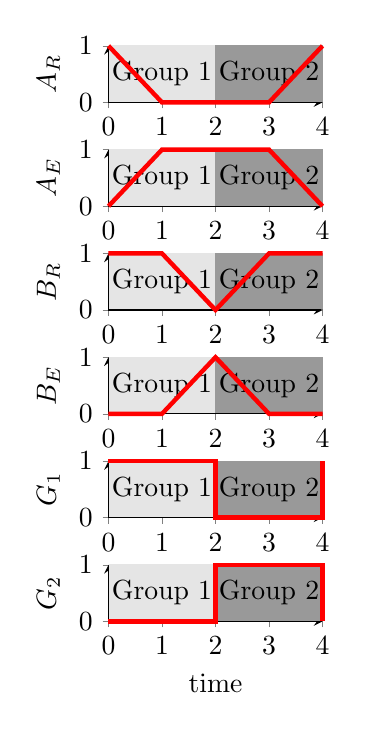
\begin{tikzpicture}
%\pgfplotsset{set layers=default}
  \begin{groupplot} [
    group style={
      group name=timeplot,
      group size=1 by 6,
      xlabels at=edge bottom,
      horizontal sep=1cm,
      vertical sep=6mm,
    }, 
    clip=false,
    height=2.3cm, width=4.3cm,
    axis line style={->},
    axis lines=left,
    xlabel={time },
    ylabel={},
    ytick={0,1},
    xtick={0,1,2,3,4},
    % grid=both,
    % xtick=\empty,
    % ytick=\XNOLL,
    % yticklabel=$x_0$,
    ]
    \nextgroupplot [ylabel={$A_R$},]
    \draw[color=black!10, fill=black!10] (axis cs: 0.02,0.02) rectangle (axis cs: 2,1);
    \node at (axis cs: 1, 0.5) {Group 1};
    \draw[color=black!40, fill=black!40] (axis cs: 2,0.02) rectangle (axis cs: 4,1);
    \node at (axis cs: 3, 0.5) {Group 2};
    \addplot[red, no marks,ultra thick,] coordinates {(0,1) (1,0) (2, 0) (3,0) (4, 1)};

    \nextgroupplot [ylabel={$A_E$},]
    \draw[color=black!10, fill=black!10] (axis cs: 0.02,0.02) rectangle (axis cs: 2,1);
    \node at (axis cs: 1, 0.5) {Group 1};
    \draw[color=black!40, fill=black!40] (axis cs: 2,0.02) rectangle (axis cs: 4,1);
    \node at (axis cs: 3, 0.5) {Group 2};
    \addplot[red, no marks,ultra thick,] coordinates {(0,0) (1,1) (2, 1) (3,1) (4, 0)};

    \nextgroupplot [ylabel={$B_R$},]
    \draw[color=black!10, fill=black!10] (axis cs: 0.02,0.02) rectangle (axis cs: 2,1);
    \node at (axis cs: 1, 0.5) {Group 1};
    \draw[color=black!40, fill=black!40] (axis cs: 2,0.02) rectangle (axis cs: 4,1);
    \node at (axis cs: 3, 0.5) {Group 2};
    \addplot[red, no marks,ultra thick,] coordinates {(0,1) (1,1) (2, 0) (3,1) (4, 1)};

    \nextgroupplot [ylabel={$B_E$},]
    \draw[color=black!10, fill=black!10] (axis cs: 0.02,0.02) rectangle (axis cs: 2,1);
    \node at (axis cs: 1, 0.5) {Group 1};
    \draw[color=black!40, fill=black!40] (axis cs: 2,0.02) rectangle (axis cs: 4,1);
    \node at (axis cs: 3, 0.5) {Group 2};
    \addplot[red, no marks,ultra thick,] coordinates {(0,0) (1,0) (2, 1) (3,0) (4, 0)};

    \nextgroupplot [ylabel={$G_1$},]
    \draw[color=black!10, fill=black!10] (axis cs: 0.02,0.02) rectangle (axis cs: 2,1);
    \node at (axis cs: 1, 0.5) {Group 1};
    \draw[color=black!40, fill=black!40] (axis cs: 2,0.02) rectangle (axis cs: 4,1);
    \node at (axis cs: 3, 0.5) {Group 2};
    \addplot[red, no marks,ultra thick,] coordinates {(0,1) (2, 1) (2,0) (4, 0) (4,1)};

    \nextgroupplot [ylabel={$G_2$},]
    \draw[color=black!10, fill=black!10] (axis cs: 0.02,0.02) rectangle (axis cs: 2,1);
    \node at (axis cs: 1, 0.5) {Group 1};
    \draw[color=black!40, fill=black!40] (axis cs: 2,0.02) rectangle (axis cs: 4,1);
    \node at (axis cs: 3, 0.5) {Group 2};
    \addplot[red, no marks,ultra thick,] coordinates {(0,0) (2, 0) (2,1) (4, 1) (4,0)};
  \end{groupplot}
\end{tikzpicture}
  \end{center}
\end{block}
\end{column}


\begin{column}{0.72\columnwidth}
\begin{block}{Control law}
\begin{center}
\begin{tabular}{|cccccc|cccc|}
\hline
\(A_R\) & \(A_E\) & \(B_R\) & \(B_E\) & \(G_11\) & \(G_2\) & \(u_A+\) & \(u_A-\) & \(u_B+\) & \(u_B-\)\\
\hline
1 & 0 & 1 & 0 & 1 & 0 &  &  &  & \\
0 & 1 & 1 & 0 & 1 & 0 &  &  &  & \\
0 & 1 & 0 & 1 & 0 & 1 &  &  &  & \\
0 & 1 & 1 & 0 & 0 & 1 &  &  &  & \\
\hline
\end{tabular}
\end{center}
\end{block}
\end{column}
\end{columns}
\end{frame}


\begin{frame}[label={sec:orgaaca8ed}]{Implementing the control law}
\begin{center}
         \begin{tikzpicture}
           \node at (-2,0.5) {+24V};
           \node at (8,0.5) {0V};
           \draw (-2,0) to[short, o-]  (-2,-7);
           \draw (8,0) to[short, o-](8,-7);
	   \draw (6, -0.5) \coil{$u_{A+}$};
           \draw (6,-2.5) \coil{$u_{A-}$};
	   \draw (6, -4.5)\coil{$u_{B+}$};
           \draw (6,-6.5)  \coil{$u_{B-}$};
      \end{tikzpicture}
\end{center}
\end{frame}


\begin{frame}[label={sec:orgf7b6a4a}]{Implementing the group transitions}
\begin{center}
         \begin{tikzpicture}
           \node at (-2,0.5) {+24V};
           \node at (8,0.5) {0V};
           \draw (-2,0) to[short, o-]  (-2,-7);
           \draw (8,0) to[short, o-](8,-7);
	   \draw (6, -0.5) \coil{$G_1$};
	   \draw (6, -4.5) \coil{$G_2$};
	   \draw (-2,-2) to[switch, label={$G_1$}] (1,-2);
	   \draw (-2,-6) to[switch, label={$G_2$}] (1,-6);
      \end{tikzpicture}
\end{center}
\end{frame}



\begin{frame}[label={sec:orgfad6fc4}]{Implementing the proximity sensor circuit}
\begin{center}
\includegraphics[height=0.9\textheight]{sensor-circuit}
\end{center}
\end{frame}
\end{document}